\providecommand{\Fun}{\operatorname{Fun}}
\providecommand{\QCat}{\mathcal{Q}\mathcal{C}at}
\providecommand{\Cat}{\mathcal{C}at}
\providecommand{\hFun}{\mathrm{h}\Fun} %
\providecommand{\HomB}{\mathrm{Hom}_{B}}
\providecommand{\HomFB}{\mathrm{Hom}_{FB}}
\providecommand{\SWarrow}{\rotatebox[origin=c]{-135}{$\Rightarrow$}} %
\providecommand{\Disc}{\mathit{Disc}}
\providecommand{\Stab}{\mathcal{S}\mathit{tab}} %
\providecommand{\Rari}{\mathit{Rari}}
\providecommand{\Lari}{\mathit{Lari}}
\providecommand{\Cart}{\mathcal{C}\mathit{art}}
\providecommand{\CoCart}{\mathit{co}\mathcal{C}\mathit{art}}
\providecommand{\Fib}{\mathcal{F}\mathit{ib}}
\providecommand{\Mod}{\mathbb{M}od}
\providecommand{\hTwoCell}[5]{\tikz[baseline=-0.8ex]{%
  \node (rvl) at (0,0) {$#1$};
  \node (rvr) at (2.9,0) {$#2$};
  \draw[->] (rvl) to[bend left=28] node[above]{$\scriptstyle #3$} (rvr);
  \draw[->] (rvl) to[bend right=28] node[below]{$\scriptstyle #5$} (rvr);
  \node at (1.45,0) {$\scriptstyle #4$};}}

\section{作为换模型函子的宇宙论双等价}\label{sec:cosmological-biequivalences-as-change-of-model-functors}

诸\trInfinityCosmos{}之间的\trBiequivalence{}被称为\trChangeOfModel{}\trFunctor。在本节中，我们列举它们的基本性质。首先，我们观察到\trCosmologicalBiequivalence{}下降为诸\trHomotopyTwoCategory{}之间的\trBiequivalence——名称由此而来：

\begin{proposition}\label{prop:homotopy-two-category-biequivalence}
一个\trCosmologicalBiequivalence{} $F\colon\mathcal{K}\Rightarrow\mathcal{L}$
诱导诸\trHomotopyTwoCategory{}之间的一个\trBiequivalence{}
$F\colon\mathfrak{h}\mathcal{K}\Rightarrow\mathfrak{h}\mathcal{L}$，也就是说，
该 2-\trFunctor
\begin{enumerate}[label=(\roman*)]
\item 依等价意义于对象上为满；并且
\item 对所有 $A$ 与 $B\in\mathcal{K}$，定义诸\trCategory{}之间的一个\trLocalEquivalence
  $\hFun(A,B)\Rightarrow\hFun(FA,FB)$。
\end{enumerate}
\end{proposition}

注意，(ii) 的诸\trLocalEquivalence{}必然具有\cref{ex:equivalence-reflects-isomorphism-classes}所列举的那些性质。

\begin{proof}
由\cref{thm:equivalences-are-equivalences}，∞-宇宙层面的\trEquivalence{}与%
2-\trCategory{}式的\trEquivalence{}相重合，这就证明了 (i)；而由\cref{lem:equiv-homotopy-equivalences}，\trHomotopyCategory{}函子
$\mathrm{h}\colon\QCat\to\Cat$ 把诸\trQuasiCategory{}之间的\trEquivalence{}送到诸\trCategory{}之间的\trEquivalence，这就证明了 (ii)。
\end{proof}

特别地，由此得出：一个\trInfinityCategory{}的\trHomotopyCategory{}在%
\trChangeOfModel{}之下不变（见\cref{ex:homotopy-category-change-of-model}）。更一般地，2-\trCategory{}之间的任何\trBiequivalence{}都诱导出多种局部与整体的双射，如下所列：

\begin{corollary}\label{cor:biequivalence-local-bijections}
考虑任何\trCosmologicalBiequivalence{} $F\colon\mathcal{K}\Rightarrow\mathcal{L}$。
\begin{enumerate}[label=(\roman*)]
\item \trBiequivalence{} $F$ 保持、反射并创造诸\trInfinityCategory{}之间的%
  \trEquivalence，并在对象的\trEquivalence{}类之间定义一个双射。
\item \trBiequivalence{} $F$ 在诸\trFunctor{}的自然\trIsomorphism{}类之间诱导出延伸 (i) 之双射的诸局部双射：选定任何一对对象 $A$ 与 $B\in\mathcal{K}$、
  任何一对 $A'$ 与 $B'\in\mathcal{L}$，以及\trEquivalence
  $a\colon A'\Rightarrow FA$ 与 $b\colon FB\Rightarrow B'$，
  映射
  \begin{rveq}\label{eq:homotopy-categories-map}
  \hFun(A,B)\Rightarrow\hFun(FA,FB)\Rightarrow\hFun(A',B')
  \end{rveq}
  在 $\mathcal{K}$ 中诸\trFunctor{} $A\to B$ 的\trIsomorphism{}类与
  $\mathcal{L}$ 中诸\trFunctor{} $A'\to B'$ 的\trIsomorphism{}类之间定义一个双射。
\item \trBiequivalence{} $F$ 在带指定边界的诸\trNaturalTransformation{}之间定义出延伸 (i) 与 (ii) 之双射的诸局部双射：选定任何一对对象 $A$ 与
  $B\in\mathcal{K}$、任何一对 $A'$ 与 $B'\in\mathcal{L}$、指定的\trEquivalence
  $a\colon A'\simeq FA$ 与 $b\colon FB\simeq B'$、
  诸\trFunctor{} $f$ 与 $g\colon A\to B$ 以及 $f'$ 与 $g'\colon A'\to B'$，还有自然\trIsomorphism
  \begin{center}
  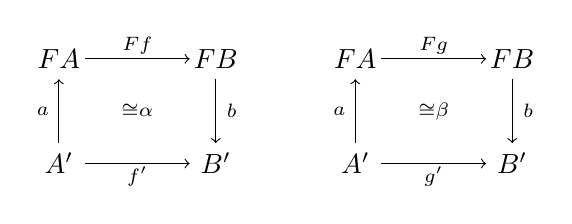
\begin{tikzpicture}[x=1.05em,y=1.05em]
    \node at (0,2.2)    {$FA$};
    \node at (5.4,2.2)  {$FB$};
    \node at (0,-1.4)   {$A'$};
    \node at (5.4,-1.4) {$B'$};
    \draw[->] (0.9,2.2) -- (4.5,2.2);
    \node at (2.7,2.66) {$\scriptstyle Ff$};
    \draw[->] (0,-0.7) -- (0,1.5);
    \node at (-0.55,0.4) {$\scriptstyle a$};
    \draw[->] (5.4,1.5) -- (5.4,-0.7);
    \node at (5.95,0.4) {$\scriptstyle b$};
    \draw[->] (0.9,-1.4) -- (4.5,-1.4);
    \node at (2.7,-1.86) {$\scriptstyle f'$};
    \node at (2.7,0.4) {$\scriptstyle\cong\alpha$};
    \begin{scope}[shift={(10.2,0)}]
      \node at (0,2.2)    {$FA$};
      \node at (5.4,2.2)  {$FB$};
      \node at (0,-1.4)   {$A'$};
      \node at (5.4,-1.4) {$B'$};
      \draw[->] (0.9,2.2) -- (4.5,2.2);
      \node at (2.7,2.66) {$\scriptstyle Fg$};
      \draw[->] (0,-0.7) -- (0,1.5);
      \node at (-0.55,0.4) {$\scriptstyle a$};
      \draw[->] (5.4,1.5) -- (5.4,-0.7);
      \node at (5.95,0.4) {$\scriptstyle b$};
      \draw[->] (0.9,-1.4) -- (4.5,-1.4);
      \node at (2.7,-1.86) {$\scriptstyle g'$};
      \node at (2.7,0.4) {$\scriptstyle\cong\beta$};
    \end{scope}
  \end{tikzpicture}
  \end{center}
  则映射 \eqref{eq:homotopy-categories-map} 在 $\mathcal{K}$ 中诸%
  \trNaturalTransformation{} $f\Rightarrow g$ 与 $\mathcal{L}$ 中诸%
  \trNaturalTransformation{} $f'\Rightarrow g'$ 之间诱导一个双射。
\end{enumerate}
\end{corollary}

\begin{proof}
\cref{lem:biequivalence-reflect-create}证明了\trCosmologicalBiequivalence{}保持、反射并创造诸\trEquivalence，其论证根本上是 2-\trCategory{}式的，请读者重访之。这一点连同\trCosmologicalBiequivalence{}的本质满性，蕴含此类\trFunctor{}在对象的\trEquivalence{}类上诱导一个双射。这就证明了 (i)。

至于 (ii)，由\cref{cor:functor-space-equivalences}，所选的\trEquivalence
$FA\simeq A'$ 与 $FB\simeq B'$ 诱导诸%
\trQuasiCategory{}之间的一个\trEquivalence
\begin{equation*}
\Fun(A,B)\xrightarrow{\ \sim\ }\Fun(FA,FB)\xrightarrow{\ \sim\ }\Fun(A',B')
\end{equation*}
它下降为诸\trHomotopyCategory{}的\trEquivalence{} \eqref{eq:homotopy-categories-map}。由于诸\trQuasiCategory{}之间的\trEquivalence{}在顶点的\trIsomorphism{}类之间诱导双射，这特别地给出诸\trFunctor{}的\trIsomorphism{}类之间的一个双射。

至于 (iii)，\trEquivalence{} \eqref{eq:homotopy-categories-map} 是\trFullyFaithful，在诸\trNaturalTransformation{} $f\Rightarrow g$ 与
$b\cdot Ff\cdot a\Rightarrow b\cdot Fg\cdot a$ 之间诱导一个双射。这一双射可沿任何所选的\trIsomorphism{} $\alpha$ 与 $\beta$ 搬运，给出 $\mathcal{K}$ 中 $\hFun(A,B)$ 内诸\trNaturalTransformation{} $f\Rightarrow g$ 与 $\mathcal{L}$ 中 $\hFun(A',B')$ 内诸\trNaturalTransformation{} $f'\Rightarrow g'$ 之间的一个双射。
\end{proof}

作为\cref{cor:biequivalence-local-bijections}的一个应用，我们现在兑现 2.3 节所作的一个承诺：确立 $(\infty,1)$-\trCategory{}的\trInfinityCosmos{}中%
\trInfinityCategory{} $A$ 与 $B$ 之间的\trInternalHom{} $B^{A}$，同 $B$ 与 $A$ 的\trUnderlyingQuasiCategory{}的单纯\trCotensor{} $B^{A_{0}}$ 之间的一个\trEquivalence。

\begin{observation}\label{obs:weak-exponentials}
即使 $(\infty,1)$-\trCategory{}的一个\trInfinityCosmos{} $\mathcal{K}$ 不是\trCartesianClosed，其\trHomotopyTwoCategory{} $\mathfrak{h}\mathcal{K}$ 在\trBicategorical{}意义下也是\trCartesianClosed——以自然\trEquivalence{}替换\cref{prop:cartesian-closure}(ii) 的诸自然\trIsomorphism。由于\cref{prop:underlying-qcat-biequivalence}的\trBiequivalence{} $(-)_{0}\colon\mathcal{K}\Rightarrow\QCat$，我们定义 $B^{A}\in\mathcal{K}$ 为任一\trUnderlyingQuasiCategory{}等价于 $B_{0}^{A_{0}}$ 的\trInfinityCategory。经由复合诸\trEquivalence
\begin{center}
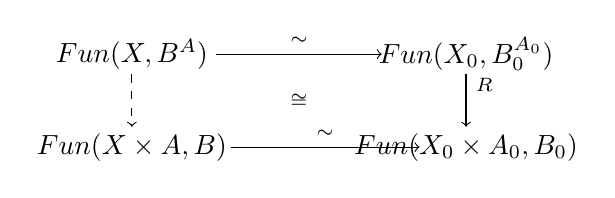
\begin{tikzpicture}[x=1.05em,y=1.05em]
  \node (a) at (0,0)    {$\Fun(X,B^{A})$};
  \node (b) at (11.5,0) {$\Fun(X_{0},B_{0}^{A_{0}})$};
  \node (c) at (0,-3.2) {$\Fun(X\times A,B)$};
  \node (d) at (11.5,-3.2) {$\Fun(X_{0}\times A_{0},B_{0})$};
  \draw[->] (2.9,0) -- node[above]{$\scriptstyle\sim$} (8.6,0);
  \draw[->] (3.4,-3.2) -- node[above]{$\scriptstyle\sim$} (9.9,-3.2);
  \draw[->,dashed] (0,-0.7) -- (0,-2.5);
  \draw[->] (11.5,-0.7) -- node[right,pos=0.2]{$\scriptstyle R$} (11.5,-2.5);
  \node at (5.75,-1.6) {$\scriptstyle\cong$};
\end{tikzpicture}
\end{center}
我们见到：对任何 $X$，$\Fun(X,B^{A})\simeq\Fun(X\times A,B)$。在定义 10.4.13
的术语中，映射 $\Fun(X,B^{A})\Rightarrow\Fun(X\times A,B)$ 是一个%
\emph{拟伪自然等价}（quasi-pseudonatural equivalence）。注意，若 $\mathcal{K}$ 是\trCartesianClosed，这一\trUniversalProperty{}表明诸弱指数等价于严格定义者。
\end{observation}

出于这一理由，\cref{prop:exponential-cotensor}的陈述不要求环境%
\trInfinityCosmos{}是\trCartesianClosed；诸指数可以事后推得存在。

\begin{proposition}\label{prop:exponential-cotensor}
在 $(\infty,1)$-\trCategory{}的一个\trInfinityCosmos{}中，对任何%
\trInfinityCategory{} $A$ 与 $B$，指数 $B^{A}$ 等价于 $B$ 与 $A$ 的\trUnderlyingQuasiCategory{}的\trCotensor{} $B^{A_{0}}$。
\end{proposition}

\begin{proof}
由\cref{cor:biequivalence-local-bijections}，诸\trCosmologicalBiequivalence{}反射诸\trInfinityCategory{}之间的\trEquivalence。于是，为证
$B^{A}\simeq B^{A_{0}}$，由\cref{prop:underlying-qcat-biequivalence}与%
\cref{cor:biequivalence-local-bijections}，只需证明 $B^{A}$ 与 $B^{A_{0}}$ 具有等价的\trUnderlyingQuasiCategory。指数与\trCotensor{}的定义性\trUniversalProperty{}提供诸\trEquivalence，它们与\trUnderlyingQuasiCategory{}函子的\trLocalEquivalence{}复合，给出所要的\trEquivalence：
\begin{equation*}
\Fun(1,B^{A})\simeq\Fun(A,B)\xrightarrow{\ \sim\ }\Fun(A_{0},B_{0})\simeq\Fun(1,B^{A_{0}})
\end{equation*}
\end{proof}

我们现在证明：\trBiequivalence{}对于\cref{prop:cosmological-preservation-properties}所考虑的诸∞-范畴论结构，在保持之外还反射并创造它们。

\begin{proposition}\label{prop:biequivalence-reflects-creates}
一个\trCosmologicalBiequivalence{} $F\colon\mathcal{K}\Rightarrow\mathcal{L}$
\begin{enumerate}[label=(\roman*)]
\item 保持、反射并创造诸\trEquivalence。
\item 保持并反射诸\trNaturalTransformation{}的可逆性，并在给定的诸\trFunctor{}之间创造诸自然\trIsomorphism。
\item 保持、反射并创造诸\trInfinityCategory{}之间的\trAdjunction，包括右伴随右逆伴随与左伴随右逆伴随。
\item 保持、反射并创造\trFiberedAdjunction{}与\trFiberedEquivalence。
\item 保持并反射离散性。
\item 保持并反射\trCommaInfinityCategory：一个\trCell{}定义 $\mathcal{K}$ 中的一个\trCommaCone，当且仅当它的像是 $\mathcal{L}$ 中的一个\trCommaCone。
\item 保持、反射并创造给定\trCospan{}之上的\trAbsoluteRightLifting{}图表与\trAbsoluteLeftLifting{}图表。
\item 保持并反射以\trSimplicialSet{}为指标的\trDiagram{}之\trLimit{}或\trColimit，并创造「一个\trInfinityCategory{}容许给定\trDiagram{}之\trLimit{}或\trColimit」这一性质。
\item 保持并反射一个\trInfinityCategory{}的稳定性与此类\trInfinityCategory{}之间的诸\trFunctor{}的正合性。
\item 保持并反射\trCartesianFibration{}与\trCocartesianFibration{}及其间的\trCartesianFunctor。
\item 保持并反射\trDiscreteCartesianFibration{}与\trDiscreteCocartesianFibration。
\item 保持并反射\trTwoSidedFibration{}及其间的\trCartesianFunctor。
\item 保持并反射\trModule{}与可表示模，并对一对固定的\trInfinityCategory{}之间的诸\trModule{}之\trEquivalence{}类诱导一个双射。
\end{enumerate}
\end{proposition}

\begin{proof}
诸保持性质已在\cref{prop:cosmological-preservation-properties}中、于较弱的假设——$F$ 只是一个\trCosmologicalFunctor——之下获证。于是只剩下处理诸性质的反射与诸∞-范畴论结构的创造。

性质 (i)、(ii) 与 (iii) 对 2-范畴之间的任何\trBiequivalence{}都成立——例如 $F\colon\mathfrak{h}\mathcal{K}\Rightarrow\mathfrak{h}\mathcal{L}$。尚未论及的那些方面留给\cref{ex:two-categorical-biequivalence}——这是一道有益的练习，可藉之熟悉双等价的 2-\trCategory{}式概念。由\cref{prop:slice-biequivalence}，(iv) 是 (i) 与 (iii) 的特例。

性质 (v) 由 (ii) 得出：若 $FE$ 是\trDiscrete，则 $\mathcal{K}$ 中任何以 $E$ 为余定义域的 2-\trCell{}在 $F$ 之下的像是可逆的，这就蕴含该 2-\trCell{}在 $E$ 中是\trInvertible。

由于 $\mathcal{K}$ 与 $\mathcal{L}$ 二者都容许\trCommaInfinityCategory，而命题 3.4.11 表明诸\trCommaSpan{}由\trTwoSidedIsofibration{}的一个\trFiberedEquivalence{}类所刻画，故 (vi) 由 (iv) 得出。

(vii) 与 (viii) 的反射性质由定理 3.5.3 得出，而创造性质由定理 3.5.12 与 (vi) 得出。然后，(ix) 可借定理 4.4.12 中任何一组等价刻画、利用 (ii) 与 (viii) 得到论证。

条目 (x) 经由定理 5.2.8 由 (iii) 与 (ii) 得出，而 (xi) 由把 (i) 应用于命题 5.5.8 所考虑的那个态射得出。性质 (xii) 类似地由定理 7.1.4(iii) 以及 (iii) 与 (ii) 得出。\trModule{}的保持与反射现在由这一点与 (v) 得出，而\trEquivalence{}类之间的双射由 (iv) 得出。\footnote{更精确的陈述出现于命题 11.1.4。}(xiii) 的可表示性陈述把 (iv) 与 (vi) 相结合，如命题 11.1.5 所详论。
\end{proof}

\begin{corollary}\label{cor:induced-biequivalences}
若 $F\colon\mathcal{K}\Rightarrow\mathcal{L}$ 是一个\trCosmologicalBiequivalence，则下列受诱导的\trCosmologicalFunctor{}都是\trBiequivalence：
\begin{enumerate}[label=(\roman*)]
\item $F\colon\Disc(\mathcal{K})\Rightarrow\Disc(\mathcal{L})$
\item $F\colon\mathcal{K}_{\top,J}\Rightarrow\mathcal{L}_{\top,J}$
  与 $F\colon\mathcal{K}_{\bot,J}\Rightarrow\mathcal{L}_{\bot,J}$
\item $F\colon\Rari(\mathcal{K})_{/B}\Rightarrow\Rari(\mathcal{L})_{/FB}$
  与 $F\colon\Lari(\mathcal{K})_{/B}\Rightarrow\Lari(\mathcal{L})_{/FB}$
\item $F\colon\Rari(\mathcal{K})\Rightarrow\Rari(\mathcal{L})$
  与 $F\colon\Lari(\mathcal{K})\Rightarrow\Lari(\mathcal{L})$
\item $F\colon\Cart(\mathcal{K})_{/B}\Rightarrow\Cart(\mathcal{L})_{/FB}$
  与 $F\colon\CoCart(\mathcal{K})_{/B}\Rightarrow\CoCart(\mathcal{L})_{/FB}$
\item $F\colon\Cart(\mathcal{K})\Rightarrow\Cart(\mathcal{L})$
  与 $F\colon\CoCart(\mathcal{K})\Rightarrow\CoCart(\mathcal{L})$
\item $F\colon\Disc\Cart(\mathcal{K})\Rightarrow\Disc\Cart(\mathcal{L})$
  与 $F\colon\Disc\CoCart(\mathcal{K})\Rightarrow\Disc\CoCart(\mathcal{L})$
\item $F\colon\Stab(\mathcal{K})\Rightarrow\Stab(\mathcal{L})$
\item $F\colon{}_{A}\Fib(\mathcal{K})_{/B}\Rightarrow{}_{FA}\Fib(\mathcal{L})_{/FB}$
\item $F\colon{}_{A}\Mod(\mathcal{K})_{/B}\Rightarrow{}_{FA}\Mod(\mathcal{L})_{/FB}$
\end{enumerate}
\end{corollary}

\begin{proof}
在每一种情形，我们都从一个\trCosmologicalBiequivalence{}出发——例如
$\mathcal{K}_{/B}\Rightarrow\mathcal{L}_{/FB}$ 或
$\mathcal{K}^{\dagger}\Rightarrow\mathcal{L}^{\dagger}$——而必须证明：%
\cref{lem:restrict-replete-cosmological}限制所得的\trCosmologicalFunctor{}仍然是诸\trCosmologicallyEmbedded{}\trInfinityCosmos{}之间的一个\trBiequivalence。每一个论证都是类似的；为具体起见，我们证明 (viii)。\cref{prop:biequivalence-reflects-creates}证明了：刻画该子\trInfinityCosmos{}的对象与 0-箭头的那种性质为任何\trBiequivalence{}所保持并反射。于是，诸\trCosmologicalFunctor{}的图表是一个\trPullback：
\begin{center}
\begin{tikzpicture}[x=1.05em,y=1.05em]
  \node at (0,1.7)    {$\Stab(\mathcal{K})$};
  \node at (8.2,1.7)  {$\Stab(\mathcal{L})$};
  \node at (0,-1.7)   {$\mathcal{K}$};
  \node at (8.2,-1.7) {$\mathcal{L}$};
  \draw[->] (2.9,1.7) -- (5.3,1.7);
  \node at (4.1,2.14) {$\scriptstyle F$};
  \draw[right hook->] (0,1.1) -- (0,-1.1);
  \draw[right hook->] (8.2,1.1) -- (8.2,-1.1);
  \draw[->] (2.2,-1.7) -- (6.0,-1.7);
  \node at (4.1,-1.26) {$\scriptstyle\sim$};
  \node at (4.1,-2.16) {$\scriptstyle F$};
  \node at (1.55,1.05) {$\scriptstyle\lrcorner$};
\end{tikzpicture}
\end{center}
故\cref{lem:pullback-cosmological-biequivalence}容许我们断言：受诱导的\trFunctor{} $\Stab(\mathcal{K})\Rightarrow\Stab(\mathcal{L})$ 是一个\trCosmologicalBiequivalence。
\end{proof}

\cref{war:composites-not-preserved}提到过一些未必为\trCosmologicalFunctor{}所保持的∞-范畴论性质。重要的是，这些概念为\trCosmologicalBiequivalence{}所保持、反射并创造。引理 11.1.7 就复合与\trExactSquare{}这两种情形证明了这一点——这两个概念居于模的\trVirtualEquipment{}之中——而我们现在处理逐点右\trExtension{}与逐点左\trExtension{}的情形。

\begin{proposition}\label{prop:pointwise-extensions-biequivalence}
一个\trCosmologicalBiequivalence{} $F\colon\mathcal{K}\Rightarrow\mathcal{L}$
保持、反射并创造逐点左\trExtension{}与逐点右\trExtension：
\begin{enumerate}[label=(\roman*)]
\item $\mathcal{K}$ 中如下形式的\trDiagram
\begin{center}
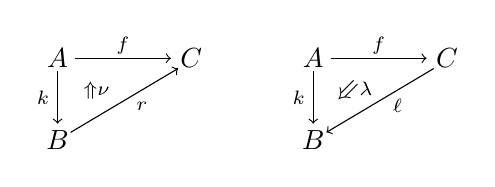
\begin{tikzpicture}[x=1.05em,y=1.05em]
  \node at (0,2.2)   {$A$};
  \node at (4.6,2.2) {$C$};
  \node at (0,-0.6)  {$B$};
  \draw[->] (0.6,2.2) -- (3.9,2.2);
  \node at (2.25,2.64) {$\scriptstyle f$};
  \draw[->] (0,1.75) -- (0,-0.05);
  \node at (-0.5,0.85) {$\scriptstyle k$};
  \draw[->] (0.45,-0.35) -- (4.15,1.85);
  \node at (2.9,0.55) {$\scriptstyle r$};
  \node at (1.35,1.1) {$\scriptstyle\Uparrow\nu$};
  \begin{scope}[shift={(8.8,0)}]
    \node at (0,2.2)   {$A$};
    \node at (4.6,2.2) {$C$};
    \node at (0,-0.6)  {$B$};
    \draw[->] (0.6,2.2) -- (3.9,2.2);
    \node at (2.25,2.64) {$\scriptstyle f$};
    \draw[->] (0,1.75) -- (0,-0.05);
    \node at (-0.5,0.85) {$\scriptstyle k$};
    \draw[->] (4.15,1.85) -- (0.45,-0.35);
    \node at (2.9,0.55) {$\scriptstyle\ell$};
    \node at (1.35,1.1) {$\scriptstyle\SWarrow\lambda$};
  \end{scope}
\end{tikzpicture}
\end{center}
定义 $\mathcal{K}$ 中的一个逐点右\trExtension{}或逐点左\trExtension，当且仅当其在 $F$ 之下的像分别定义 $\mathcal{L}$ 中的一个逐点右\trExtension{}或逐点左\trExtension。
\item 若 $\mathcal{K}$ 中的诸\trFunctor{} $f\colon A\to C$ 与 $k\colon A\to B$ 使得 $Ff\colon FA\to FC$ 在 $\mathcal{L}$ 中沿 $Fk\colon FA\to FB$ 容许一个逐点右\trExtension{}或逐点左\trExtension，则 $f$ 在 $\mathcal{K}$ 中分别沿 $k$ 容许一个逐点右\trExtension{}或逐点左\trExtension，且其在 $F$ 之下的像同构于 $\mathcal{L}$ 中的相应数据。
\end{enumerate}
\end{proposition}

为解释证明的想法，我们首先证明\trCosmologicalBiequivalence{}保持并反射右\trExtension；它们也创造右\trExtension，但这在逐点情形可以同样容易地证明，逐点情形随后讨论。

首先设 $\nu\colon rk\Rightarrow f$ 是 $\mathcal{K}$ 中的一个右\trExtension。为证其像定义 $\mathcal{L}$ 中的一个右\trExtension，我们必须证明：对所有 $d\colon FB\to FC$，映射
\begin{equation*}
\begin{gathered}
\hFun(FB,FC)(d,Fr)\xrightarrow{\ F\nu\circ\ }\hFun(FA,FC)(d\cdot Fk,Ff)\\
d\overset{\gamma}{\Rightarrow}Fr\longmapsto d\cdot Fk\overset{\gamma Fk}{\Rightarrow}Fr\cdot Fk\overset{F\nu}{\Rightarrow}Ff
\end{gathered}
\end{equation*}
在诸 2-\trCell{}的集合上定义一个双射。由\cref{cor:biequivalence-local-bijections}(ii)，存在 $\mathcal{K}$ 中一个\trFunctor{} $c\colon B\to C$ 连同一个自然\trIsomorphism{} $\delta\colon d\cong Fc$。由\cref{cor:biequivalence-local-bijections}(iii)，$F$ 的应用与同 $\delta$ 的复合定义一个双射
\begin{equation*}
\begin{gathered}
\hFun(B,C)(c,r)\xrightarrow{\ F\ }\hFun(FB,FC)(Fc,Fr)\xrightarrow{\ -\circ\delta\ }\hFun(FB,FC)(d,Fr)\\
c\overset{\alpha}{\Rightarrow}r\longmapsto Fc\overset{F\alpha}{\Rightarrow}Fr\longmapsto d\overset{\delta}{\Rightarrow}Fc\overset{F\alpha}{\Rightarrow}Fr
\end{gathered}
\end{equation*}
从可逆 2-\trCell{} $\delta Fk\colon d\cdot Fk\cong Fc\cdot Fk$ 出发可定义一个类似的双射。由于 $\nu\colon rk\Rightarrow f$ 是一个右\trExtension，与 $\nu$ 的复合诱导出它自己的一族双射。从函数的如下交换方块——其中三个已知为双射——我们见到：$F\nu\colon Fr\cdot Fk\Rightarrow Ff$ 是 $\mathcal{L}$ 中的一个右\trExtension，如所断言。
\begin{center}
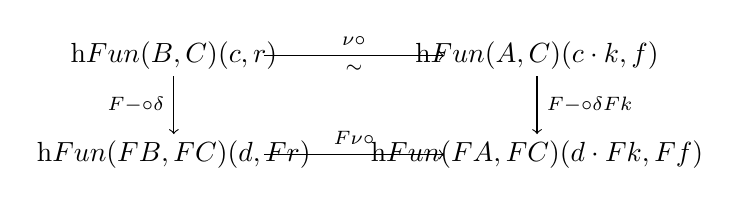
\begin{tikzpicture}[x=1.05em,y=1.05em]
  \node (a) at (0,0)     {$\hFun(B,C)(c,r)$};
  \node (b) at (12.5,0)  {$\hFun(A,C)(c\cdot k,f)$};
  \node (c) at (0,-3.4)  {$\hFun(FB,FC)(d,Fr)$};
  \node (d) at (12.5,-3.4) {$\hFun(FA,FC)(d\cdot Fk,Ff)$};
  \draw[->] (3.1,0) -- node[above]{$\scriptstyle\nu\circ$} node[below]{$\scriptstyle\sim$} (9.3,0);
  \draw[->] (0,-0.7) -- node[left]{$\scriptstyle F-\circ\delta$} (0,-2.7);
  \draw[->] (12.5,-0.7) -- node[right]{$\scriptstyle F-\circ\delta Fk$} (12.5,-2.7);
  \draw[->] (3.1,-3.4) -- node[above]{$\scriptstyle F\nu\circ$} (9.3,-3.4);
\end{tikzpicture}
\end{center}

现在设 $F\nu\colon Fr\cdot Fk\Rightarrow Ff$ 是 $\mathcal{L}$ 中的一个右\trExtension。为见 $\nu\colon rk\Rightarrow f$ 是 $\mathcal{K}$ 中的一个右\trExtension，注意对任何\trFunctor{} $c\colon B\to C$，有函数的如下交换方块
\begin{center}
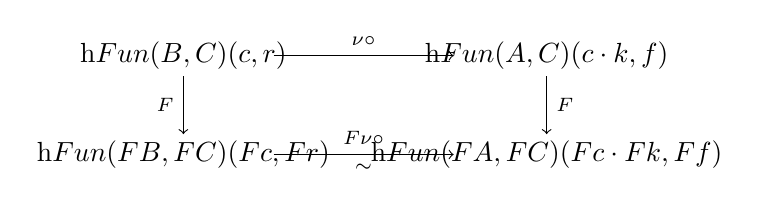
\begin{tikzpicture}[x=1.05em,y=1.05em]
  \node (a) at (0,0)     {$\hFun(B,C)(c,r)$};
  \node (b) at (12.5,0)  {$\hFun(A,C)(c\cdot k,f)$};
  \node (c) at (0,-3.4)  {$\hFun(FB,FC)(Fc,Fr)$};
  \node (d) at (12.5,-3.4) {$\hFun(FA,FC)(Fc\cdot Fk,Ff)$};
  \draw[->] (3.1,0) -- node[above]{$\scriptstyle\nu\circ$} (9.3,0);
  \draw[->] (0,-0.7) -- node[left]{$\scriptstyle F$} (0,-2.7);
  \draw[->] (12.5,-0.7) -- node[right]{$\scriptstyle F$} (12.5,-2.7);
  \draw[->] (3.1,-3.4) -- node[above]{$\scriptstyle F\nu\circ$} node[below]{$\scriptstyle\sim$} (9.3,-3.4);
\end{tikzpicture}
\end{center}
其中三个已知为双射。这就证明了 $\nu\colon rk\Rightarrow f$ 具有右\trExtension{}的\trUniversalProperty。

逐点右\trExtension{}的论证本质相同，其中我们额外利用「\trCommaInfinityCategory{}为\trCosmologicalFunctor{}所保持且在\trEquivalence{}之下不变」这一事实（练习 3.4.iv 之义）。

\begin{proof}
我们全程使用\cref{thm:pointwise-right-extensions}(ii) 所给的逐点右\trExtension{}的 2-范畴式定义。想法是利用\cref{cor:biequivalence-local-bijections}所提供的诸局部双射。

设 $\nu\colon rk\Rightarrow f$ 是 $\mathcal{K}$ 中的一个逐点右\trExtension。我们必须证明：对 $\mathcal{L}$ 中每个 $h\colon L\to FB$，图表
\begin{center}
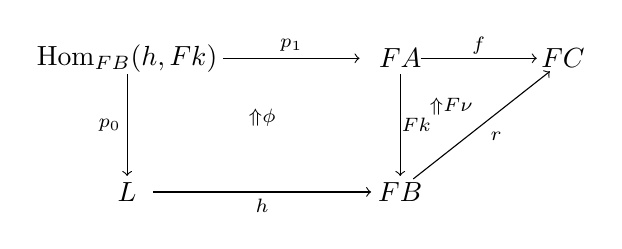
\begin{tikzpicture}[x=1.05em,y=1.05em]
  \node at (0,2.6)    {$\HomFB(h,Fk)$};
  \node at (9.4,2.6)  {$FA$};
  \node at (15.0,2.6) {$FC$};
  \node at (0,-2.0)   {$L$};
  \node at (9.4,-2.0) {$FB$};
  \draw[->] (3.3,2.6) -- (8.0,2.6);
  \node at (5.65,3.04) {$\scriptstyle p_{1}$};
  \draw[->] (10.1,2.6) -- (14.1,2.6);
  \node at (12.1,3.04) {$\scriptstyle f$};
  \draw[->] (0,2.05) -- (0,-1.45);
  \node at (-0.6,0.3) {$\scriptstyle p_{0}$};
  \draw[->] (9.4,2.05) -- (9.4,-1.45);
  \node at (9.95,0.3) {$\scriptstyle Fk$};
  \draw[->] (0.9,-2.0) -- (8.4,-2.0);
  \node at (4.65,-2.46) {$\scriptstyle h$};
  \draw[->] (9.85,-1.55) -- (14.55,2.15);
  \node at (12.7,-0.1) {$\scriptstyle r$};
  \node at (4.65,0.55) {$\scriptstyle\Uparrow\phi$};
  \node at (11.15,0.95) {$\scriptstyle\Uparrow F\nu$};
\end{tikzpicture}
\end{center}
是 $\mathcal{L}$ 中的一个右\trExtension{}图表，也就是说：对所有 $d\colon L\to FC$\footnote{原书印作「$d\colon L\Rightarrow FC$」（双杆），而 p.400 同语境印作「$d\colon FB\to FC$」（单杆），前后摇摆不一，此处按 0-箭头记号体系统一作单杆。——译者注}，映射
\begin{equation*}
\begin{gathered}
\hFun(L,FC)(d,Fr\cdot h)\xrightarrow{\ F\nu p_{1}\circ F\phi\circ\ }\hFun(\HomFB(h,Fk))(dp_{0},Ff\cdot p_{1})\\
d\overset{\varsigma}{\Rightarrow}Fr\cdot h\longmapsto dp_{0}\overset{\varsigma p_{0}}{\Rightarrow}Fr\cdot hp_{0}\overset{Fr\phi}{\Rightarrow}Fr\cdot Fk\cdot p_{1}\overset{F\nu p_{1}}{\Rightarrow}Ff\cdot p_{1}
\end{gathered}
\end{equation*}
定义诸 2-\trCell{}集合之间的一个双射。由\cref{cor:biequivalence-local-bijections}(i)，存在一个\trInfinityCategory{} $K\in\mathcal{K}$ 与一支\trEquivalence{} $e\colon L\Rightarrow FK$；由\cref{cor:biequivalence-local-bijections}(ii)，存在诸\trFunctor{} $b\colon K\to B$ 与 $c\colon K\to C$ 以及自然\trIsomorphism{} $\beta\colon Fb\cdot e\cong h$ 与 $\delta\colon d\cong Fc\cdot e$。由\cref{cor:biequivalence-local-bijections}(iii)，$F$ 的应用与同 $e$、$\beta$、$\delta$ 的复合定义一个双射\footnote{原书此双射式右端印作「$\Fun(L,FC)(d,Fr\cdot h)$」，缺同伦范畴函子之字头（同式左端实印「$\hFun(K,C)(c,rb)$」，带 $\mathrm{h}$）；按上下文此式诸项皆为同伦范畴间之态射，应为 $\hFun(L,FC)(d,Fr\cdot h)$ 之漏排，此处径补。——译者注}
\begin{equation*}
\begin{gathered}
\hFun(K,C)(c,rb)\xrightarrow{\ \sim\ }\hFun(L,FC)(d,Fr\cdot h)\\
c\overset{\gamma}{\Rightarrow}rb\longmapsto d\overset{\delta}{\Rightarrow}Fc\cdot e\overset{F\gamma e}{\Rightarrow}Fr\cdot Fb\cdot e\overset{Fr\beta}{\Rightarrow}Fr\cdot h
\end{gathered}
\end{equation*}

由于 $\nu\colon rk\Rightarrow f$ 是 $\mathcal{K}$ 中的一个逐点右\trExtension，图表
\begin{rveq}\label{eq:pointwise-right-extension-diagram}
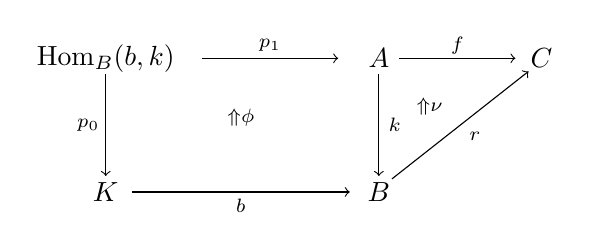
\begin{tikzpicture}[x=1.05em,y=1.05em]
  \node at (0,2.6)    {$\HomB(b,k)$};
  \node at (9.4,2.6)  {$A$};
  \node at (15.0,2.6) {$C$};
  \node at (0,-2.0)   {$K$};
  \node at (9.4,-2.0) {$B$};
  \draw[->] (3.3,2.6) -- (8.0,2.6);
  \node at (5.65,3.04) {$\scriptstyle p_{1}$};
  \draw[->] (10.1,2.6) -- (14.1,2.6);
  \node at (12.1,3.04) {$\scriptstyle f$};
  \draw[->] (0,2.05) -- (0,-1.45);
  \node at (-0.6,0.3) {$\scriptstyle p_{0}$};
  \draw[->] (9.4,2.05) -- (9.4,-1.45);
  \node at (9.95,0.3) {$\scriptstyle k$};
  \draw[->] (0.9,-2.0) -- (8.4,-2.0);
  \node at (4.65,-2.46) {$\scriptstyle b$};
  \draw[->] (9.85,-1.55) -- (14.55,2.15);
  \node at (12.7,-0.1) {$\scriptstyle r$};
  \node at (4.65,0.55) {$\scriptstyle\Uparrow\phi$};
  \node at (11.15,0.95) {$\scriptstyle\Uparrow\nu$};
\end{tikzpicture}
\end{rveq}
也是一个（逐点）右\trExtension，定义出双射
\begin{equation*}
\begin{gathered}
\hFun(K,C)(c,rb)\xrightarrow{\ \simeq\ }\hFun(\HomB(b,k),C)(cp_{0},fp_{1})\\
c\overset{\gamma}{\Rightarrow}rb\longmapsto cp_{0}\overset{\gamma p_{0}}{\Rightarrow}rbp_{0}\overset{r\phi}{\Rightarrow}rkp_{1}\overset{\nu p_{1}}{\Rightarrow}fp_{1}
\end{gathered}
\end{equation*}

由练习 3.4.iv 有一个等价\hspace{-1pt}$y\colon\HomFB(h,Fk)\Rightarrow\HomFB(Fb,Fk)\cong Fb\,\HomB(b,k)$ 居于 $e\times\mathrm{id}\colon L\times FA\Rightarrow FK\times FA$ 之上。
由\cref{cor:biequivalence-local-bijections}(iii)，$F$ 的应用与同 $y$、$\beta$、$\delta$ 的复合定义出函数的如下交换方块中右侧的那个双射
\begin{center}
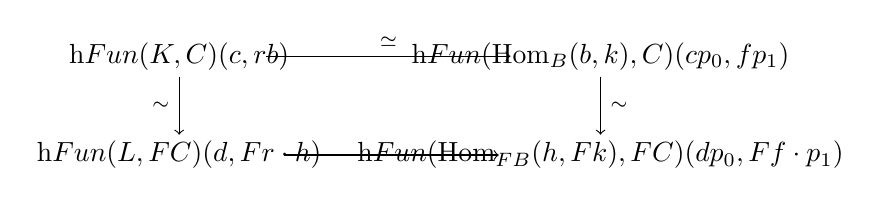
\begin{tikzpicture}[x=1.05em,y=1.05em]
  \node (a) at (0,0)     {$\hFun(K,C)(c,rb)$};
  \node (b) at (14.5,0)  {$\hFun(\HomB(b,k),C)(cp_{0},fp_{1})$};
  \node (c) at (0,-3.4)  {$\hFun(L,FC)(d,Fr\cdot h)$};
  \node (d) at (14.5,-3.4) {$\hFun(\HomFB(h,Fk),FC)(dp_{0},Ff\cdot p_{1})$};
  \draw[->] (3.0,0) -- node[above]{$\scriptstyle\simeq$} (11.4,0);
  \draw[->] (0,-0.7) -- node[left]{$\scriptstyle\sim$} (0,-2.7);
  \draw[->] (14.5,-0.7) -- node[right]{$\scriptstyle\sim$} (14.5,-2.7);
  \draw[->] (3.6,-3.4) -- (11.0,-3.4);
\end{tikzpicture}
\end{center}
于是 $\mathcal{L}$ 中我们的粘贴图表是一个右\trExtension{}图表，如所欲证。

为见逐点右\trExtension{}被反射，我们必须在「$F\nu\colon Fr\cdot Fk\Rightarrow Ff$ 是 $\mathcal{L}$ 中一个逐点右\trExtension{}图表」这一假设之下证明：\eqref{eq:pointwise-right-extension-diagram} 是 $\mathcal{K}$ 中的一个右\trExtension{}图表。对任何\trFunctor{} $c\colon K\to C$，有函数的如下交换方块：
\begin{center}
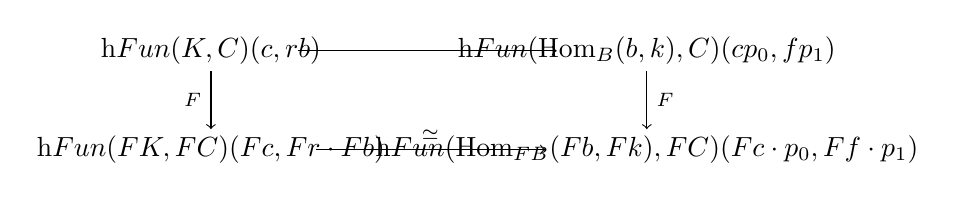
\begin{tikzpicture}[x=1.05em,y=1.05em]
  \node (a) at (0,0)     {$\hFun(K,C)(c,rb)$};
  \node (b) at (15.0,0)  {$\hFun(\HomB(b,k),C)(cp_{0},fp_{1})$};
  \node (c) at (0,-3.4)  {$\hFun(FK,FC)(Fc,Fr\cdot Fb)$};
  \node (d) at (15.0,-3.4) {$\hFun(\HomFB(Fb,Fk),FC)(Fc\cdot p_{0},Ff\cdot p_{1})$};
  \draw[->] (3.0,0) -- (11.9,0);
  \draw[->] (0,-0.7) -- node[left]{$\scriptstyle F$} (0,-2.7);
  \draw[->] (15.0,-0.7) -- node[right]{$\scriptstyle F$} (15.0,-2.7);
  \draw[->] (3.6,-3.4) -- node[above]{$\scriptstyle\simeq$} (11.5,-3.4);
\end{tikzpicture}
\end{center}
由于\trCommaSquare{}为\trCosmologicalFunctor{}所保持，底部映射是一个双射——由 $F$ 的应用所定义的诸竖直函数亦然。于是，$\nu\colon r\cdot k\Rightarrow f$ 满足 $\mathcal{K}$ 中逐点右\trExtension{}的\trUniversalProperty。

最后，为见逐点右\trExtension{}图表为\trCosmologicalBiequivalence{}所创造，设给定 $\mathcal{L}$ 中一个逐点右\trExtension{}图表
\begin{center}
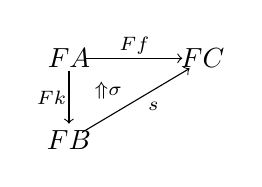
\begin{tikzpicture}[x=1.05em,y=1.05em]
  \node at (0,2.2)   {$FA$};
  \node at (4.6,2.2) {$FC$};
  \node at (0,-0.6)  {$FB$};
  \draw[->] (0.6,2.2) -- (3.9,2.2);
  \node at (2.25,2.64) {$\scriptstyle Ff$};
  \draw[->] (0,1.75) -- (0,-0.05);
  \node at (-0.6,0.85) {$\scriptstyle Fk$};
  \draw[->] (0.45,-0.35) -- (4.15,1.85);
  \node at (2.9,0.55) {$\scriptstyle s$};
  \node at (1.35,1.1) {$\scriptstyle\Uparrow\sigma$};
\end{tikzpicture}
\end{center}
由\cref{cor:biequivalence-local-bijections}，存在一个\trFunctor{} $r\colon B\to C$ 连同\trIsomorphism{} $\alpha\colon s\cong Fr$ 与一支\trNaturalTransformation{} $\nu\colon rk\Rightarrow f$，后者在双射
\begin{equation*}
\begin{gathered}
\hFun(A,C)(rk,f)\xrightarrow{\ F(-)\circ\alpha Fk\ }\hFun(FA,FC)(s\cdot Fk,Ff)\\
rk\overset{\nu}{\Rightarrow}f\longmapsto s\cdot Fk\overset{\sigma}{\Rightarrow}Ff
\end{gathered}
\end{equation*}
之下被映射为 $\sigma$。由于 $F\nu$ 同构于 $\mathcal{L}$ 中一个逐点右\trExtension{}图表，它是 $\mathcal{L}$ 中一个逐点右\trExtension{}图表；而由于逐点右\trExtension{}图表为\trCosmologicalBiequivalence{}所反射，$\nu$ 展示 $r$ 为 $f$ 沿 $k$ 的一个逐点右\trExtension，如所断言。
\end{proof}

立即得自定义 9.4.7 与引理 9.5.6：
\begin{corollary}\label{cor:weighted-limits-biequivalence}
\trCosmologicalBiequivalence{}保持、反射并创造以\trInfinityCategory{}为指标的\trDiagram{}之（加权）\trLimit{}与\trColimit。\qed
\end{corollary}

\subsection*{练习}

\begin{exercise}\label{ex:homotopy-category-change-of-model}
设 $F\colon\mathcal{K}\Rightarrow\mathcal{L}$ 是一个\trCosmologicalBiequivalence。请证明：$F$ 对任何\trInfinityCategory{} $A\in\mathcal{K}$ 都诱导诸\trHomotopyCategory{}之间的一个\trEquivalence{} $\mathrm{h}A\rightsquigarrow\mathrm{h}FA$（见\cref{def:homotopy-category-infinity-category}）。
\end{exercise}

\begin{exercise}\label{ex:two-categorical-biequivalence}
考虑一个 2-\trFunctor{} $F\colon\mathcal{C}\to\mathcal{D}$，它一如\cref{prop:homotopy-two-category-biequivalence}那样定义一个\trBiequivalence。请证明：
\begin{enumerate}[label=(\roman*)]
\item $\mathcal{C}$ 中的一个 2-\trCell{}
  \hTwoCell{A}{B}{f}{\Downarrow\alpha}{g}
  是\trInvertible，当且仅当 $F\alpha$ 在 $\mathcal{D}$ 中是\trInvertible。
\item 一个 1-\trCell{} $u\colon A\to B$ 在 $\mathcal{C}$ 中容许一个\trLeftAdjoint，当且仅当 $Fu\colon FA\to FB$ 在 $\mathcal{D}$ 中容许一个\trLeftAdjoint，此时 $F$ 保持该\trAdjunction。
\end{enumerate}
\end{exercise}

\begin{exercise}\label{ex:cartesian-closed-exponentials}
请证明：\trCartesianClosed\trInfinityCosmos{}之间的\trCosmologicalBiequivalence{}在等价意义下保持指数对象。
\end{exercise}

